%\documentclass[compress,t,11pt]{beamer}
\documentclass[handout,compress,t,11pt]{beamer}
\usetheme[]{metropolis}           % Use metropolis theme
\usefonttheme{serif}
\definecolor[named]{Gray}{RGB}{111,112,114}
\definecolor[named]{DarkGray}{RGB}{48,48,48}
\definecolor[named]{Cardinal}{RGB}{179,22,34}
\usepackage[T1]{fontenc}
\usepackage[altbullet]{lucidabr}
\usepackage{textcomp}
\usepackage{upquote} % needed to make straight quotes work in listings
\usepackage{listgolang}
\usepackage{mathtools}
\usepackage{comment}
\usepackage{tikz}
\usepackage{tikzsymbols}
 \usetikzlibrary{trees,shapes,plotmarks,arrows,er,automata,petri,topaths,positioning}
\usepackage{pifont}
\usepackage{clrscode}
\usepackage{setspace}
\usepackage{soul}
\usepackage{hyperref}

\setbeamercolor{palette primary}{fg=white,bg=Cardinal}
\setbeamercolor{palette secondary}{fg=white,bg=Gray}
\setbeamercolor{palette tertiary}{fg=white,bg=Cardinal}
\setbeamercolor{palette quaternary}{fg=white,bg=Gray}
\setbeamercolor{palette sidebar primary}{fg=white,bg=Cardinal}
\setbeamercolor{palette sidebar secondary}{fg=white,bg=Gray}
\setbeamercolor*{titlelike}{fg=Cardinal}
\setbeamercolor{structure}{fg=Gray}
\setbeamercolor{title separator}{fg=Cardinal}
\setbeamercolor{alerted text}{fg=Cardinal}
\setbeamercolor{reversed}{fg=Cardinal,bg=black}

\newcommand{\card}[1]{\ensuremath{\left|#1\right|}}
\newcommand{\norm}[1]{\ensuremath{\|#1\|}}

\title[Programming in Go]{\bf Programming in Go\\ Lesson 3: Structs, Networking, Testing \& Tools}
\author{Matt Holiday} 
\institute[CP]{Cardinal Peak}
\date{30 April 2019} 
%\titlegraphic{\hfill
\includegraphics[width=.25\textwidth,height=.25\textheight]{cp-logo-2x.png}}
\titlegraphic{
\begin{tikzpicture}[overlay, remember picture,scale=0.4]
\node[at=(current page.north east), anchor=north east] (a) {};
\node[below left = 0.1cm and 0.1cm of a] (b)
{
\includegraphics[width=.25\textwidth,height=.25\textheight]{cp-logo-2x.png}};
\node[below left=2.56cm and 2.9cm of b]
{
\includegraphics[width=.1\textwidth]{go-logo.png}};
\end{tikzpicture}}

\setbeamerfont{footline}{series=\bfseries\selectfont}
\setbeamersize{text margin left=12pt,text margin right=12pt}
\linespread{1.0}
\metroset{block=fill}

\hypersetup{
    colorlinks=true,
    linkcolor=Cardinal,
    filecolor=magenta,      
    urlcolor=blue,
}

\begin{document}
\frame{\titlepage} 

%\section{Introduction}
\begin{frame}[fragile]
    \frametitle{Lesson \#2}
    What we'll cover today:
    \begin{itemize}
    \item Homework \#2
    \item Structs
    \item JSON
    \item Simple web clients \& servers
    \item Unit tests
    \item Static analysis tools
    \end{itemize}
\end{frame}

% =================================================================================

\begin{frame}[fragile]
\frametitle{Homework \#2}
\begin{golang}
package main

import (
    "bytes"
    "fmt"
    "os"
    "strings"

    "golang.org/x/net/html"
)
\end{golang}
\end{frame}

\begin{frame}[fragile]
\frametitle{Homework \#2}
\begin{golang}
var raw = `
<!DOCTYPE html>
<html>
  <body>
    <h1>My First Heading</h1>
      <p>My first paragraph.</p>
      <p>HTML images are defined with the img tag:</p>
      <img src="xxx.jpg" width="104" height="142">
  </body>
</html>`
\end{golang}
\end{frame}

\begin{frame}[fragile]
\frametitle{Homework \#2}
\begin{golang}
func main() {
    doc, err := html.Parse(bytes.NewReader([]byte(raw)))

    if err != nil {
        fmt.Fprintf(os.Stderr, "parse failed: %s\n", err)
        os.Exit(-1)
    }

    words, pics := countWordsAndImages(doc)

    fmt.Printf("%d words and %d images\n", words, pics)
}

// outputs "14 words and 1 images"
\end{golang}
\end{frame}

\begin{frame}[fragile]
\frametitle{Homework \#2}
\begin{golang}
func countWordsAndImages(doc *html.Node) (int, int) {
    var words, images int

    visit(doc, &words, &images)

    return words, images
}
\end{golang}
\end{frame}

\begin{frame}[fragile]
\frametitle{Homework \#2}
\begin{golang}
func visit(n *html.Node, words, pics *int) {
    // if it's an element node then see what tag it has

    if n.Type == html.TextNode {
        *words += len(strings.Fields(n.Data))
    } else if n.Type == html.ElementNode && n.Data == "img" {
        *pics++
    }

    // then visit all the children using recursion

    for c := n.FirstChild; c != nil; c = c.NextSibling {
        visit(c, words, pics)
    }
}
\end{golang}
\end{frame}

% =================================================================================

\section{Structs}
\begin{frame}[fragile]
    \frametitle{Structs}
    We've already seen a couple of aggregate types:
    \begin{itemize}
        \item slices \& arrays group a sequence of the same type
        \item maps use one type to index a collection of another type
    \end{itemize}
    \vspace{\baselineskip}
    A \verb|struct| is an aggregate of possibly disparate types \par
\begin{golang}
type Employee struct {
    Name   string
    Number int
    Boss   *Employee
    Hired  time.Time
}
\end{golang}
    \vspace{\baselineskip}
    Notice that we can have a pointer to the type we're defining \par
\end{frame}

\begin{frame}[fragile]
    \frametitle{Structs}
    In other languages it's a ``record'' (using database terminology) \par
    \vspace{0.2\baselineskip}
    It's parts are called ``fields'' and each must have a unique name \par
    \vspace{\baselineskip}
    Access to the fields is with ``dot'' notation 
\begin{golang}
employees := make(map[string]*Employee)

var matt = Employee{
    Name:   "Matt",
    Number: 72,
    Boss:   employees["Bernard"],
    Hired:  time.Date(2017, 12, 9, 16, 30, 0, 0, time.UTC),
}

employees[matt.Name] = &matt
\end{golang}
\end{frame}

\begin{frame}[fragile]
    \frametitle{Struct initialization}
With names, selected fields can be initialized \par
\vspace{0.4\baselineskip}
The others default to ``zero''
\vspace{0.4\baselineskip}
\begin{golang}
employees := make(map[string]*Employee)

var matt = Employee{
    Name:   "Matt",
    Number: 72,
    Hired:  time.Date(2017, 12, 9, 16, 30, 0, 0, time.UTC),
}

employees[matt.Name] = &matt
\end{golang}
\vspace{0.4\baselineskip}
Here \verb|matt.Boss| is left to the default value \verb|nil|
\end{frame}

\begin{frame}[fragile]
    \frametitle{Anonymous Structs}
    Anonymous structs are possible:
\begin{golang}
var album = struct {
    title  string
    artist string
    year   int,
    copies int,
}{
    "The White Album",
    "The Beatles",
    1968,
    10000000,
}
\end{golang}
\vspace{\baselineskip}
Initialization can be done without names by setting all fields in the correct order \par
\end{frame}

\begin{frame}[fragile]
    \frametitle{Struct compatibility}
    Two \verb|struct| types are compatible if
    \begin{itemize}
        \item the fields have the same types and names
        \item in the same order
        \item and the same tags (more on this later)
    \end{itemize}
    \vspace{\baselineskip}
    A \verb|struct| may be copied or passed as a parameter in its entirety \par
    \vspace{\baselineskip}
    A \verb|struct| is comparable if all its fields are comparable \par
    \vspace{\baselineskip}
    The zero value for a \verb|struct| is ``zero'' for each field in turn
\end{frame}

\begin{frame}[fragile]
    \frametitle{Passing structs}
    Structs are passed by value unless a pointer is used
\begin{golang}
var white album

func soldAnother(a album) {
    // oops
    a.copies++
}

func soldAnother(a *album) {
    // what you intended
    a.copies++
}
\end{golang}
\vspace{\baselineskip}
Note that ``dot'' notation works on pointers too, same as \verb|(*a).copies|
\end{frame}

\begin{frame}[fragile]
    \frametitle{Struct gotcha}
    Here's an annoying little issue in Go:
\begin{golang}
// Note -- not a pointer anymore
employees := make(map[string]Employee)

var matt Employee{
    Name:   "Matt",
    Number: 72,
    Boss:   &bernard,
    Hired:  time.Date( . . . ),
}

employees[matt.Name] = matt

employees["Matt"].Number++         // can't do this
\end{golang}
\vspace{0.4\baselineskip}
A \verb|map| entry is not addressable; \href{https://github.com/golang/go/issues/3117}{issue \#3117}
\end{frame}

\begin{frame}[fragile]
    \frametitle{Make the zero value useful}
    {\setstretch{1.2}
    ``It is usually desirable that the zero value be a natural or sensible default. \par
     For example, in \verb|bytes.Buffer|, the initial value of the struct is a 
     ready-to-use empty buffer, and the zero value of \verb|sync.Mutex| . . . \\
     is a ready-to-use unlocked mutex.'' ({\em GOPL} \S4.4)\\}
\end{frame}

\begin{frame}[fragile]
    \frametitle{Empty structs}
    A \verb|struct| with no fields is useful; it takes up no space \par
    \vspace{0.4\baselineskip}
    These examples draw on future material: \par
\begin{golang}
// a set type (instead of bool)

var isPresent map[int]struct{}

// a way to warn on bad struct copies (go vet)

type noCopy struct{}

func (*noCopy) Lock()   {}
func (*noCopy) Unlock() {}

// a very cheap channel type

done := make(chan struct{})
\end{golang}
\end{frame}

% =================================================================================

\section{Struct Tags and JSON}
\begin{frame}[fragile]
    \frametitle{Struct tags}
    Tags are a part of a \verb|struct| definition captured by the compiler \par
    \vspace{0.4\baselineskip}
    They are available to code that uses {\em reflection}
\begin{golang}
type Response struct {
    Page  int      `json:"page"`
    Words []string `json:"words,omitempty"`
}
\end{golang}
    \vspace{\baselineskip}
    Sometimes multiple tags are appropriate, separated by a space
\begin{golang}
type Response struct {
    Page  int      `json:"page" db:"page"`
    Words []string `json:"words,omitempty" db:"words"`
}
\end{golang}
\end{frame}

\begin{frame}[fragile]
    \frametitle{Reflection in action: JSON support}
    The JSON package in Go uses reflection on Go objects
    \vspace{0.4\baselineskip}
\begin{golang}
r := &Response{Page: 1, Words: []string{"up", "lo", "an"}}

j, _ := json.Marshal(r)              // ignoring errs
fmt.Println(string(j))

var r2 Response

json.Unmarshal(j, &r2)               // ignoring errs
fmt.Printf("%#v\n", r2)

// {"page":1,"words":["up","lo","an"]}
// main.Response{Page:1, Words:[]string{"up", "lo", "an"}}
\end{golang}
\end{frame}

\begin{frame}[fragile]
    \frametitle{Reflection in action: JSON support}
    ``omitempty'' causes a nil object to be ignored by \verb|Marshal|
    \vspace{0.4\baselineskip}
\begin{golang}
r := &Response{Page: 1, Words: []string{}}

j, _ := json.Marshal(r)              // ignoring errs
fmt.Println(string(j))

var r2 Response

json.Unmarshal(j, &r2)               // ignoring errs
fmt.Printf("%#v\n", r2)

// {"page":1}
// main.Response{Page:1, Words:[]string(nil)}
\end{golang}
\end{frame}

\begin{frame}[fragile]
    \frametitle{Struct tags have many uses}
    Tags can also be used in conjunction with SQL queries
    \vspace{0.4\baselineskip}
\begin{golang}
import "github.com/jmoiron/sqlx"

type item struct {
	Name string `db:"name"`
	When string `db:"created"`
}

func PutStats(db *sqlx.DB, item *item) error {
	stmt := `INSERT INTO items (name, created) 
             VALUES (:name, :created);`
	_, err := db.NamedExec(stmt, item)

	return err
}
\end{golang}
\end{frame}

\begin{frame}[fragile]
    \frametitle{Struct tag gotcha}
    Only {\bf exported} (capitalized) field names are convertible
    \vspace{0.4\baselineskip}
\begin{golang}
import "github.com/jmoiron/sqlx"
    
type item struct {
	Name string `db:"name"`
	when string `db:"created"` // oops
}

func PutItem(db *sqlx.DB, item *item) error {
	stmt := `INSERT INTO items (name, created) 
             VALUES (:name, :created);`

    // fails, missing when
	_, err := db.NamedExec(stmt, item)

	return err
}
\end{golang}
\end{frame}

% =================================================================================

\section{Networking with HTTP}

% \begin{frame}[fragile]
%     \frametitle{Fun with HTTP}
%     \begin{center}
%     
\includegraphics[height=.9\textheight]{http-error-code-joke.jpg}
%     \end{center}
% \end{frame}

\begin{frame}[fragile]
    \frametitle{Go network libraries}
    The Go standard library has many packages for making web servers: \par
    \vspace{\baselineskip}
    That includes:
    \begin{itemize}
        \item client \& server sockets
        \item route multiplexing
        \item HTTP and HTML, including HTML templates
        \item JSON and other data formats
        \item cryptographic security
        \item SQL database access
        \item compression utilities
        \item image generation
    \end{itemize}
    \vspace{0.4\baselineskip}
    There are also lots of 3rd-party packages with improvements \par
\end{frame}

\begin{frame}[fragile]
    \frametitle{A very short web server}
    A simple web server is almost a one-line program \par
\begin{golang}
package main

import (
	"fmt"
    "log"
	"net/http"
)

func handler(w http.ResponseWriter, r *http.Request) {
    fmt.Fprintf(w, "Hello, world! from %s\n", r.URL.Path[1:])
}

func main() {
    http.HandleFunc("/", handler)
    log.Fatal(http.ListenAndServe(":8080", nil))
}
\end{golang}
\end{frame}

\begin{frame}[fragile]
    \frametitle{A very short web server}
    Go run a web server:
    \begin{center}
    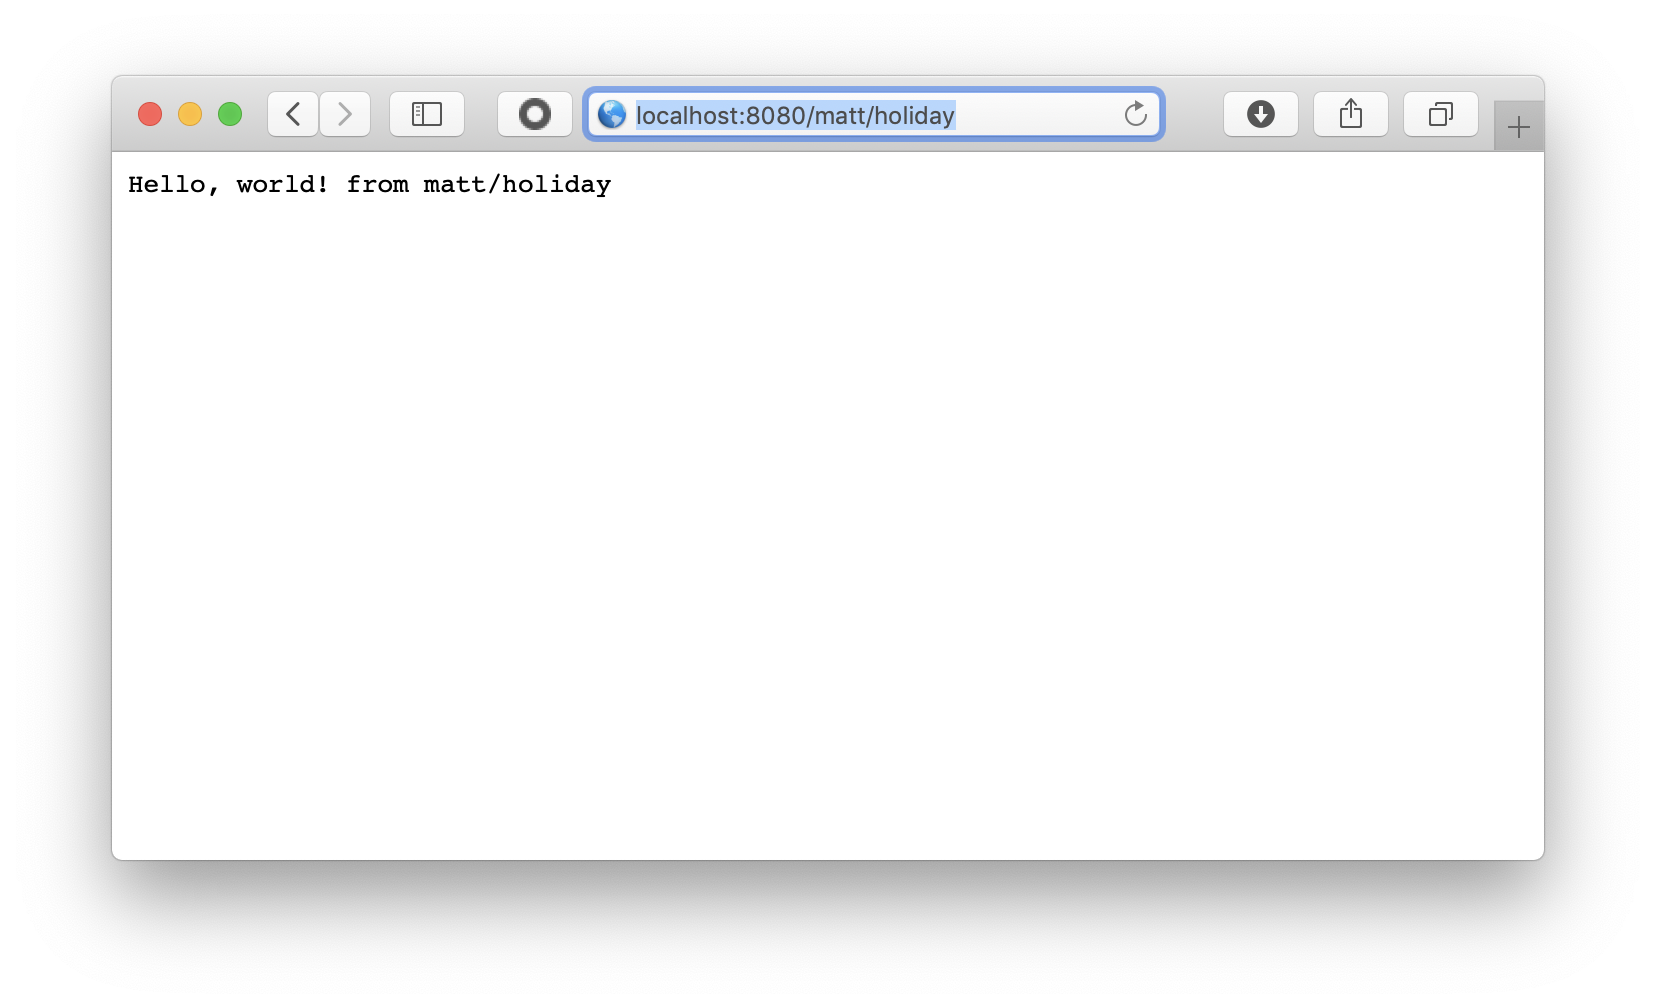
\includegraphics[width=.9\textwidth]{hello-world-http.png}
    \end{center}
\end{frame}

\begin{frame}[fragile]
    \frametitle{Go HTTP design}
    An HTTP handler function is an instance of an interface
\begin{golang}
type Handler interface {
	ServeHTTP(ResponseWriter, *Request)
}
    
type HandlerFunc func(ResponseWriter, *Request)

func (f HandlerFunc) ServeHTTP(w ResponseWriter, r *Request) {
    f(w, r)
}

// handler matches type HandlerFunc and so interface Handler
// so the HTTP framework can call ServeHTTP on it

func handler(w http.ResponseWriter, r *http.Request) {
    fmt.Fprintf(w, "Hello, world! from %s\n", r.URL.Path[1:])
}
\end{golang}
\end{frame}

\begin{frame}[fragile]
    \frametitle{A very short web client}
    A simple web client takes a little bit more \par
\begin{golang}
package main

import ("fmt"; "io/ioutil"; "net/http"; "os")

func main() {
	resp, _ := http.Get("http://localhost:8080/" + os.Args[1])
	defer resp.Body.Close()

	if resp.StatusCode == http.StatusOK {
		body, _ := ioutil.ReadAll(resp.Body)
		fmt.Println(string(body))
	}
}

// $ go run client.go matt/holiday
// Hello, world! from matt/holiday
\end{golang}
\end{frame}

\begin{frame}[fragile]
    \frametitle{A simple JSON REST client}
\begin{golang}
package main

import ("fmt"; "io/ioutil"; "net/http")
const url = "https://jsonplaceholder.typicode.com"

func main() {
	resp, _ := http.Get(url + "/todos/1")
	defer resp.Body.Close()

	if resp.StatusCode == http.StatusOK {
		body, _ := ioutil.ReadAll(resp.Body)
		fmt.Println(string(body))
	}
}

// $ go run client.go
// {"userId": 1, "id": 1, "title": "delectus aut autem", 
//  "completed": false}
\end{golang}
\end{frame}

\begin{frame}[fragile]
    \frametitle{A simple JSON REST client}
\begin{golang}
package main

import (
    "encoding/json"
    "fmt"
    "io/ioutil"
    "net/http"
)

type todo struct {
    UserID    int    `json:"userID"`
    ID        int    `json:"id"`
    Title     string `json:"title"`
    Completed bool   `json:"completed"`
}

const base = "https://jsonplaceholder.typicode.com"
\end{golang}
\end{frame}

\begin{frame}[fragile]
    \frametitle{A simple JSON REST client}
\begin{golang}
func main() {
    var item todo

	resp, _ := http.Get(base + "/todos/1")

	defer resp.Body.Close()

    body, _ := ioutil.ReadAll(resp.Body)

    _ := json.Unmarshal(body, &item)

    fmt.Printf("%#v\n", item)
}

// $ go run client.go
// main.todo{UserID:1, ID:1, Title:"delectus aut autem", 
//           Completed:false}
\end{golang}
\end{frame}

\begin{frame}[fragile]
    \frametitle{Serving from a template}
\begin{golang}
package main

import (
	"encoding/json"
	"html/template"
	"io/ioutil"
	"log"
	"net/http"
)

type todo struct {
	UserID    int    `json:"userID"`
	ID        int    `json:"id"`
	Title     string `json:"title"`
	Completed bool   `json:"completed"`
}

const base = "https://jsonplaceholder.typicode.com/"
\end{golang}
\end{frame}

\begin{frame}[fragile]
    \frametitle{Serving from a template}
\begin{golang}
var form = `
<h1>Todo #{{.ID}}</h1>
<div>{{printf "User %d" .UserID}}</div>
<div>{{printf "%s (completed: %t)" .Title .Completed}}</div>`

func handler(w http.ResponseWriter, r *http.Request) {
	var item todo

	resp, _ := http.Get(base + r.URL.Path[1:])
	defer resp.Body.Close()
	body, _ := ioutil.ReadAll(resp.Body)
	_ = json.Unmarshal(body, &item)

	tmpl := template.New("mine")

	tmpl.Parse(form)
	tmpl.Execute(w, item)
}
\end{golang}
\end{frame}

\begin{frame}[fragile]
    \frametitle{Serving from a template}
\begin{golang}
func main() {
	http.HandleFunc("/", handler)
	log.Fatal(http.ListenAndServe(":8080", nil))
}
\end{golang}
\vspace{-0.4\baselineskip}
\begin{center}
    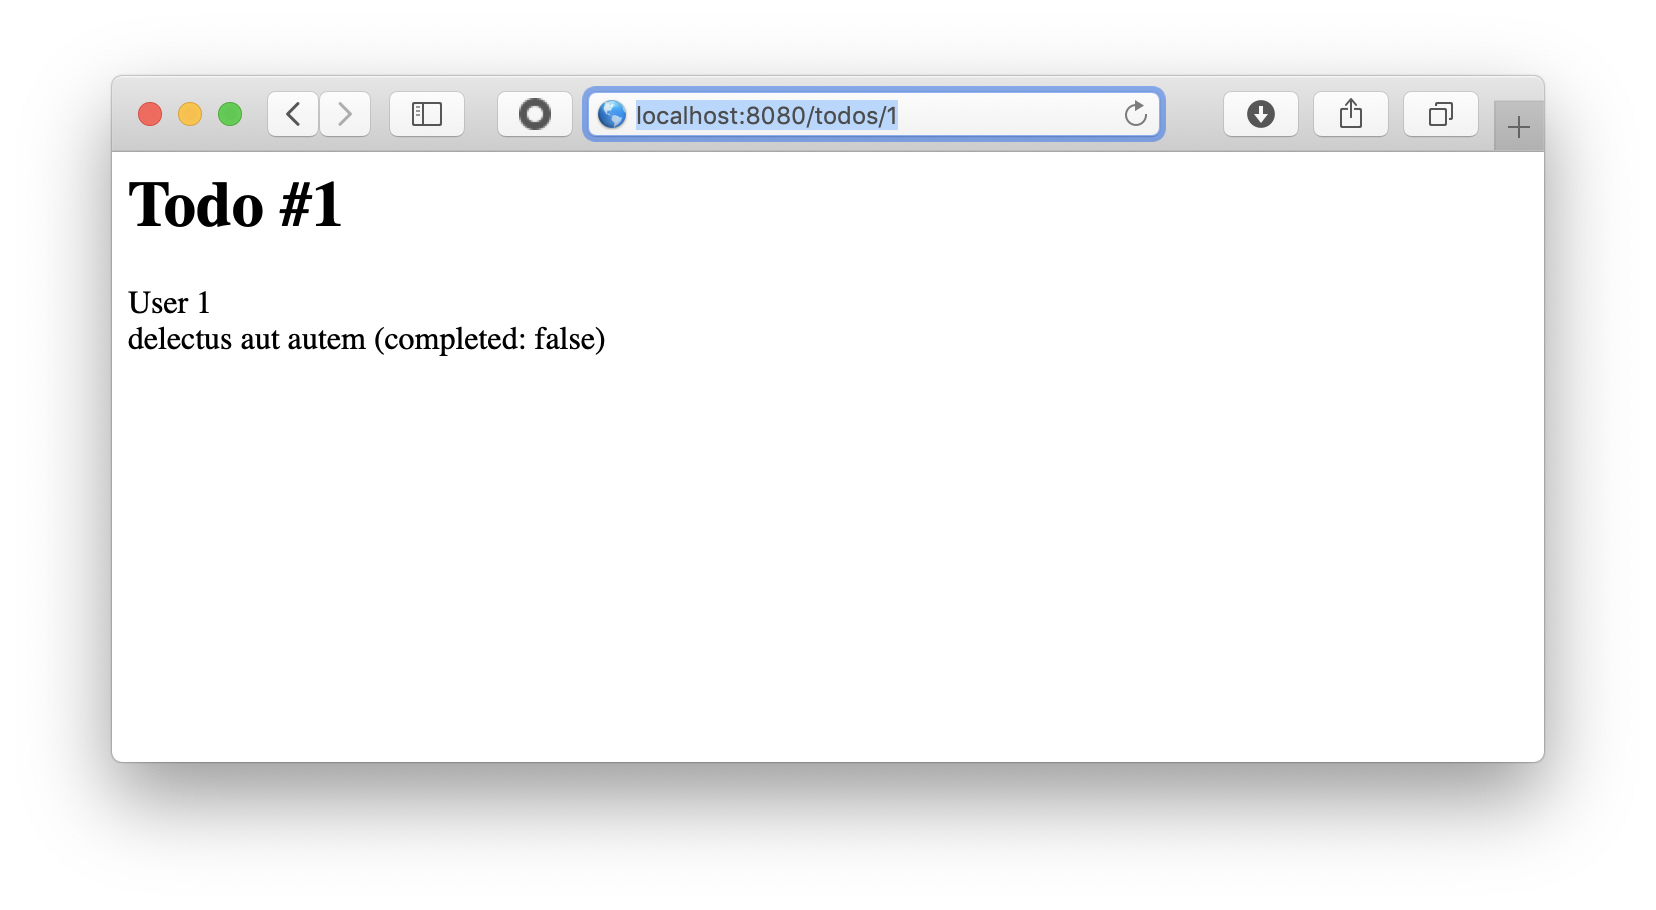
\includegraphics[width=.9\textwidth]{todos-1.png}
\end{center}
\end{frame}

\begin{frame}[fragile]
    \frametitle{Serving up an error}
\begin{golang}
func handler(w http.ResponseWriter, r *http.Request) {
	var item todo

	resp, _ := http.Get(base + r.URL.Path[1:])
	defer resp.Body.Close()

    if resp.StatusCode != http.StatusOK {
        http.NotFound(w, r)
        return
    }

	body, _ := ioutil.ReadAll(resp.Body)
	_ = json.Unmarshal(body, &item)

	tmpl := template.New("mine")
	tmpl.Parse(form)
	tmpl.Execute(w, item)
}
\end{golang}
\end{frame}

\begin{frame}[fragile]
    \frametitle{Serving up a wiki}
    See the Golang article \href{https://golang.org/doc/articles/wiki/}%
    {Writing Web Applications} \par
    \vspace{\baselineskip}
    The tutorial includes:
    \begin{itemize}
        \item creating a data structure with load and save methods
        \item using the net/http package to build web applications
        \item using the html/template package to process HTML templates
        \item using the regexp package to validate user input
        \item using closures
    \end{itemize}
\end{frame}


% =================================================================================

\section{Testing in Go}
\begin{frame}[fragile]
    \frametitle{Go unit tests}
    Go has standard tools and conventions for unit testing \par
    \vspace{0.4\baselineskip}
    Test files end with \verb|_test.go| and have \verb|TestXXX| functions \par
    \vspace{0.4\baselineskip}
    Typically they're in a separate directory, but not necessarily \par
    \vspace{0.4\baselineskip}
    You run tests with \verb|go test| \par
\begin{verbatim}
go test ./test
ok  	bvi/test	56.841s
go test ./pkg/acedb
ok  	bvi/pkg/acedb	(cached)
\end{verbatim}
    \vspace{0.4\baselineskip}
    Tests aren't run if the source wasn't changed since the last test
\end{frame}

\begin{frame}[fragile]
    \frametitle{Unit test functions}
    Test functions have the same signature using \verb|testing.T| 
\begin{golang}

func TestCrypto(t *testing.T) {
	uuid := "650b5cc5-5c0b-4c00-ad97-36b08553c91d"
	key1 := "75abbabc1f9f8d28d55200b43fd95962"
	key2 := "75abbabc1f9f8d28d66200b43fd95962"

	ct, err := secrets.MakeAppKey(key1, uuid)

	if err != nil {
		t.Errorf("make failed: %s", err)
	}
    
    . . .
}
\end{golang}
    \vspace{0.4\baselineskip}
    Errors are reported through that parameter and fail the test
\end{frame}

%% ADD MORE ON UTs

% =================================================================================

\section{Static Analysis}

\begin{frame}[fragile]
    \frametitle{Static analysis}
    ``Static'' means we're not running the program \par
    \vspace{0.4\baselineskip}
    We can analyze source files and find many possible defects
    \begin{itemize}
        \item style issues
        \item security issues
        \item things that might compile but be wrong
        \item excessive code complexity
        \item inefficient structure layout
    \end{itemize}
    \vspace{\baselineskip}
    We can also automatically 
    \begin{itemize}
        \item reformat code
        \item update import lists
    \end{itemize}
\end{frame}

\begin{frame}[fragile]
    \frametitle{Start clean, stay clean}
    Cruft and ``technical debt'' can build up pretty quickly \par
    \vspace{0.4\baselineskip}
    Not all code smells will be found by these static tools \par
    \vspace{3\baselineskip}
    Pay heed to the tools on every file save and every commit \par
    \vspace{0.4\baselineskip}
    Put little bits of time in every day to prevent lots of work later
\end{frame}

\begin{frame}[fragile]
    \frametitle{Gofmt and Goimports}
    \verb|gofmt| will put your code in standard form (spacing, indentation) \par
    \vspace{0.4\baselineskip}
    It will notify you if something was changed \par
    \vspace{0.4\baselineskip}
    \verb|goimports| will do that and also update import lists \par
    \vspace{4\baselineskip}
    {\bf The standard practice is to run one or the other on\\
    every save in your IDE/editor (as a 
    \href{https://blog.golang.org/go-fmt-your-code}{save file hook})} \par
    \vspace{\baselineskip}
    They can also be run as a 
    \href{https://github.com/golang/go/blob/master/misc/git/pre-commit}%
    {pre-commit hook} in your local repo
\end{frame}

\begin{frame}[fragile]
    \frametitle{Golint}
    \verb|golint| will check for non-format style isses, for example: 
    \begin{itemize}
        \item exported names should have comments for \verb|godoc|
        \item names shouldn't have \verb|under_scores| or be in \verb|ALLCAPS|
        \item \verb|panic| shouldn't be used for normal error handling
        \item the error flow should be indented, the happy path not
        \item variable declarations shouldn't have redundant type info
    \end{itemize}
    \vspace{3\baselineskip}
    The ``rules'' are based on \href{https://golang.org/doc/effective_go.html}{Effective Go} and
     Google's\\ \href{https://github.com/golang/go/wiki/CodeReviewComments}{Go Code Review Comments}
\end{frame}

\begin{frame}[fragile]
    \frametitle{Go vet}
    \verb|go vet| will find some issues the compiler won't \par
    \vspace{\baselineskip}
    For example, it will report suspicious ``printf'' format strings \par
    \vspace{\baselineskip}
    It can flag cases were you've accidentally copied a mutex type \par
    \vspace{\baselineskip}
    It can find cases of ``shadowing'' that might be in error \\
    (Go 1.12 makes this part harder to run, but still worth it)\par
    \vspace{2\baselineskip}
    Run it before you build
\end{frame}

\begin{frame}[fragile]
    \frametitle{Other tools}
    There are too many tools to list \par
    \vspace{0.4\baselineskip}
    \verb|gosec| looks for possible security issues \par
    \vspace{0.4\baselineskip}
    \verb|ineffasign| finds assignments that are ``ineffective'' (shadowed?) \par
    \vspace{0.4\baselineskip}
    \verb|gocyclo| reports high \href{https://en.wikipedia.org/wiki/Cyclomatic_complexity}%
    {cyclomatic complexity} in functions\par
    \vspace{2\baselineskip}
    Treat these things as {\bf warnings} because there are false positives \par
    \vspace{\baselineskip}
    Many of these can be run by the uber-tool \href{https://github.com/alecthomas/gometalinter}%
    {\tt metalinter} \par
    (I let the \href{https://www.jetbrains.com/go/}{GoLand} IDE run it on every save)
\end{frame}

\begin{frame}[fragile]
    \frametitle{Download with go get}
\begin{verbatim}
    go get golang.org/x/lint/golint
    go get golang.org/x/tools/cmd/goimports
    go get github.com/fzipp/gocyclo
    go get github.com/gordonklaus/ineffassign
    go get github.com/securego/gosec/cmd/gosec
    go get honnef.co/go/tools/cmd/staticcheck
\end{verbatim}
\end{frame}

% =================================================================================

\section{Homework}
\begin{frame}[fragile]
    \frametitle{Homework \#3}
    Exercise 4.12 from {\em GOPL:} fetching from the web \par
    \vspace{0.4\baselineskip}
{\small \setstretch{1.1} The popular web comic ``xkcd'' has a JSON interface. 
For example, a request to 
\href{https://xkcd.com/571/info.0.json}{https://xkcd.com/571/info.0.json}
produces a detailed description of comic 571, one of many favorites. Download 
each URL (once!) and build an offline index. Write a tool xkcd that, using this 
index, prints the URL {\em and date} of each comic whose {\em transcript} 
matches a search string provided on the command line. \\}
\begin{center}
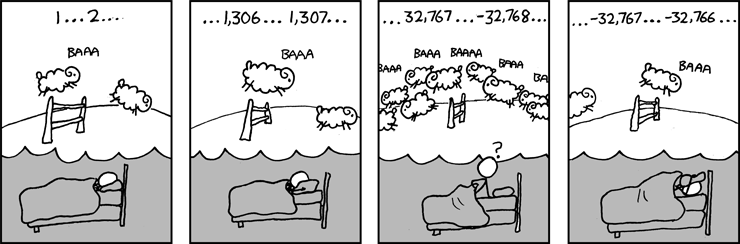
\includegraphics[width=.6\textwidth]{cant_sleep.png}
\end{center}
\end{frame}
\begin{frame}[fragile]
    \frametitle{Homework \#3}
    What the raw data looks like:
{\small
\begin{verbatim}
{
 "month":      "4", 
 "num":        571, 
 "link":       "", 
 "year":       "2009", 
 . . . 
 "transcript": "[[Someone is in bed, . . . long int.", 
 "img":        "https://imgs.xkcd.com/comics/cant_sleep.png", 
 "title":      "Can't Sleep",
 "day":        "20"
}
\end{verbatim}}
For the query ``Someone is in bed'' we get the URL and date: 
\verb|https://xkcd.com/571/ 4/20/2009|
\end{frame}

\end{document}
